\normaltrue \difficilefalse \tdifficilefalse
\correctiontrue
%\UPSTIidClasse{11} % 11 sup, 12 spé
%\newcommand{\UPSTIidClasse}{11}

\exer{Pince Robovolc  $\star$ \label{CHS:03:B2:16:71}}
%% CCP MP 2007
\setcounter{question}{0}\marginnote{\xpComp{CHS}{03}}%\UPSTIcompetence[2]{B2-16}
\index{Compétence CHS-03}\index{Compétence B2-16}

\index{Robovolc}
\index{Hyperstatisme}

\ifcorrection
\else
\marginnote{\textbf{Pas de corrigé pour cet exercice.}}
\fi


\question{Calculer l'hyperstatisme du mécanisme global de la pince (\autoref{fig_23}).}
\ifprof

Le graphe de liaisons est donné figure suivante. 

\begin{center}
\includegraphics[width=7cm]{71_01_Cor}
\end{center}

\marginnote{Si la pince est en position serrée, il n'y a pas de mobilité << utile >>. }
\begin{itemize}
\item \textbf{Dans le plan}, on a $m=1$ : rotation de 6 autour de l'axe $\axe{Q}{z_p}$.
\item $I_c = 6\times 1 + 1 \times 1 + 1 \times 2 = 9$ (6 pivots, 1 glissière et 1 ponctuelle dans le plan);
\item $E_c = 3 \times 3 = 9$
\item $h=m-I_c+E_c = 1-9+9 = 1$. 
\end{itemize}
\begin{itemize}
\item \textbf{Dans l'espace}, on a $m=2$ : rotations de 6 autour de l'axe $\axe{Q}{z_p}$ et $\axe{Q}{y_p}$.
\item $I_c = 6\times 1 + 1 \times 1 + 1 \times 5 = 12$ (6 pivots, 1 glissière et 1 ponctuelle );
\item $E_c = 6 \times 3 = 18$
\item $h=2-I_c+E_c = 1-12+18 = 7$. 
\end{itemize}
\else
\fi

\ifprof
\else
\begin{figure}[H]
\centering
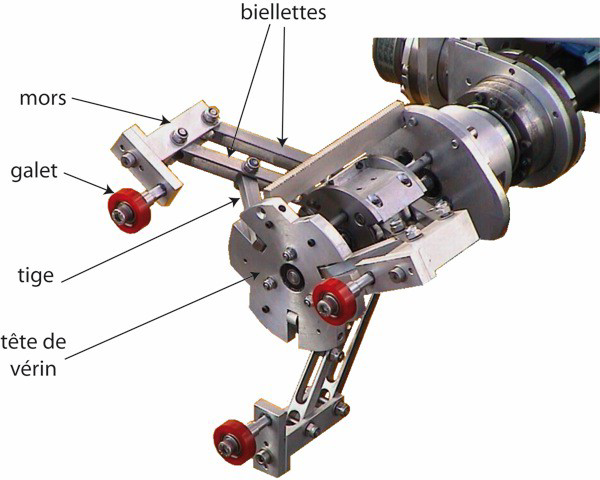
\includegraphics[width=.45\linewidth]{fig_23a.png}
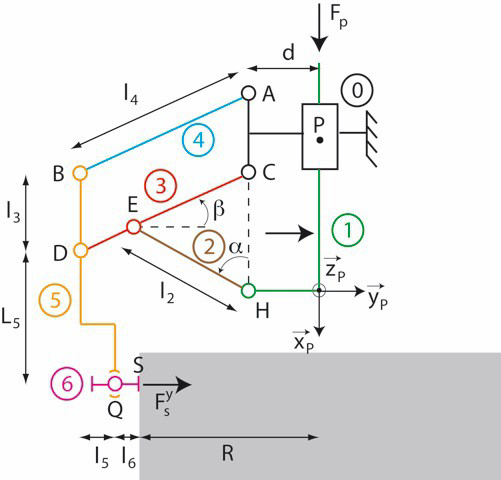
\includegraphics[width=.45\linewidth]{fig_23b.png}
\caption{Pince utilisée sur le système ROBOVOLC et schéma cinématique associé \label{fig_23}}
\end{figure} 
\fi 

\ifprof
\else
\ifcolle
\else
\marginnote{
\begin{solution}
 \begin{enumerate}
\item $h=0$.
%\item $h=8$.
%\item .
 \end{enumerate}
 \end{solution}i}
 \fi

\marginnote{Corrigé  voir \ref{CHS:03:B2:16:71}.}
\fi